\section{Prototyping}

Nachdem ein Gesamtkonzept geplant wurde, wird nun möglichst viel Prototyping durchgeführt. Das Ziel ist es, zu testen, ob das ermittelte Konzept funktionieren könnte oder ob es überarbeitet werden muss. So kann mit den Risiken, die im vorhergehenden Kapitel ermittelt wurden, besser umgegangen werden.

\subsection{...}

\subsection{Kürzester Weg finden}

Da es nur 8 Knoten im Graph gibt, wurde von Anfang an vermutet, dass die Geschwindigkeit des Algorithmus vernachlaessigt werden kann.

Um zu ueberpruefen, dass diese These stimmt, wurde ein traditioneller Dijkstra Algorithmus in Python implementiert. Dabei wurde von einem Knoten der kuerzeste Weg zu allen anderen Knoten im vorgegebenen Graphen mit 8 Knoten berechnet. Die Zeit dafuer wurde gestoppt und ausgegeben:

\begin{figure}[H]
\centering
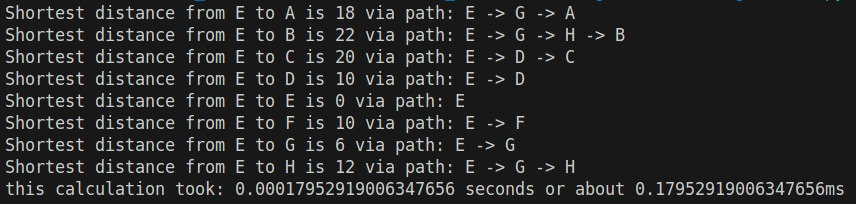
\includegraphics[width=\textwidth -30mm]{assets/informatik-prototyp/dijkstra-time.jpeg}
\caption{Dijkstra Zeitmessung}
\label{fig:dijkstra-time}
\end{figure}

Um den kuerzesten Pfad acht mal zu berechnen wurden ungefaehr 18 
 Es war jedoch wichtig, dass der Algorithmus moeglichst lightweight ist, da nur eine beschraenkte Rechenkraft zu Verfuegung steht.


\subsection{Bilderkennung}

\subsection{Simulator}

Das Erarbeiten des Konzeptes des Simulators, der Implementierung und des Gebrauchs wird in diesem Kapitel festgehalten.

Nach der Nutzwertanalyse war das grundlegende Konzept klar und es konnte mit der Implementierung begonnen werden.

- GitHub, Issues sammeln, Festlegen Git ettiquete (aka MRs)

- Struktur mit Klassen (ERD?): Robot, Reader, Calculator, GUI

- Roboter liest Graph, ueberprueft Nodes und Barrieren

- Calculator holt kürzester Weg, Roboter geht zu nächsten Node

- Poetry

- Die einzelnen Kanten werden identifiziert mit Sortierung

- GUI Roboter bewegt sich
